%\documentclass[PhD]{iitmdiss}
%\documentclass[MS]{iitmdiss}
%\documentclass[MTech]{iitmdiss}
%\documentclass[BTech]{iitmdiss}
\documentclass[DD]{iitmdiss}
\usepackage{times}
 \usepackage{t1enc}

\usepackage{graphicx}
%\usepackage{epstopdf}
\usepackage[driverfallback=dvipdfm,pdfusetitle]{hyperref} % hyperlinks for references.
\hypersetup{
	pdfsubject={Dept. of Engg. Design, IIT Madras, B.Tech M.Tech Dual Degree Project Report},
	pdfkeywords={IITM,Dual Degree,Report}
}
\usepackage{amsmath} % easier math formulae, align, subequations \ldots

\begin{document}

%%%%%%%%%%%%%%%%%%%%%%%%%%%%%%%%%%%%%%%%%%%%%%%%%%%%%%%%%%%%%%%%%%%%%%
% Title page

\title{Infrastructure Agnostic\\
	 Cloud Computing Platform for Programming Education}

\author{Muhammed Shahidh K, ED12B031}

\date{MAY 2017}
\department{ENGINEERING DESIGN}

%\nocite{*}
\maketitle

%%%%%%%%%%%%%%%%%%%%%%%%%%%%%%%%%%%%%%%%%%%%%%%%%%%%%%%%%%%%%%%%%%%%%%
% Certificate
\certificate

\vspace*{0.5in}

\noindent This is to certify that the thesis titled {\bf Infrastructure Agnostic Cloud Computing Platform for Programming Education}, submitted by {\bf Muhammed Shahidh K, ED12B031}, 
  to the Indian Institute of Technology Madras, for
the award of the dual degree of {\bf Bachelor of Technology and Master of Technology}, is a bona fide
record of the research work done by him under our supervision.  The
contents of this thesis, in full or in parts, have not been submitted
to any other Institute or University for the award of any degree or
diploma.

\vspace*{1.5in}

\begin{singlespacing}
\hspace*{-0.25in}
\parbox{2.5in}{
\noindent {\bf Dr.~Gaurav~Raina} \\
\noindent Research Guide \\ 
\noindent Assistant Professor \\
\noindent Dept. of Electrical Engineering\\
\noindent IIT Madras, 600036 \\
} 
\hspace*{1.0in} 
\parbox{2.5in}{
\noindent {\bf Dr.~Asokan~Thondiyath} \\
\noindent Research Guide \\ 
\noindent Professor \\
\noindent Dept. of Engineering Design\\
\noindent IIT Madras, 600036 \\
}  
\end{singlespacing}
\vspace*{0.25in}
\noindent Place: Chennai\\
Date: 21st May 2017 


%%%%%%%%%%%%%%%%%%%%%%%%%%%%%%%%%%%%%%%%%%%%%%%%%%%%%%%%%%%%%%%%%%%%%%
% Acknowledgements
\acknowledgements

<will update>

%%%%%%%%%%%%%%%%%%%%%%%%%%%%%%%%%%%%%%%%%%%%%%%%%%%%%%%%%%%%%%%%%%%%%%
% Abstract

\abstract

\noindent KEYWORDS: \hspace*{0.5em} \parbox[t]{4.4in}{Cloud Computing, Virtualisation, Docker, Kubernetes, Education, Programming}

\vspace*{24pt}

\noindent The project showcases a scalable online programming platform which can be used to teach computer programming languages to students, by just using a web browser. The underlying architecture and use of virtualisation technology makes the platform infrastructure agnostic and hence can be deployed on to any cloud provider as well as bare metal. Using container runtime environments such as Docker, the platform can be configured to run any programming language and library. Further a PoC was developed and deployed for nearly 1,00,000 users for India's biggest MOOC (Massive Online Open Course) - IMAD (Introduction to Modern Application Development).

\pagebreak

%%%%%%%%%%%%%%%%%%%%%%%%%%%%%%%%%%%%%%%%%%%%%%%%%%%%%%%%%%%%%%%%%
% Table of contents etc.

\begin{singlespace}
\tableofcontents
\thispagestyle{empty}

\listoftables
\addcontentsline{toc}{chapter}{LIST OF TABLES}
\listoffigures
\addcontentsline{toc}{chapter}{LIST OF FIGURES}
\end{singlespace}


%%%%%%%%%%%%%%%%%%%%%%%%%%%%%%%%%%%%%%%%%%%%%%%%%%%%%%%%%%%%%%%%%%%%%%
% Abbreviations
\abbreviations

\noindent 
\begin{tabbing}
xxxxxxxxxxx \= xxxxxxxxxxxxxxxxxxxxxxxxxxxxxxxxxxxxxxxxxxxxxxxx \kill
\textbf{IITM}   \> Indian Institute of Technology Madras \\
\textbf{MOOC} \> Massive Open Online Course \\
\textbf{K8S} \> Kubernetes \\
\textbf{VM} \> Virtual Machine \\
\textbf{GCE} \> Google Compute Engine \\
\textbf{GKE} \> Google Container Engine \\
\textbf{IP} \> Internet Protocol \\
\textbf{HTTP} \> Hyper Text Transfer Protocol \\
\textbf{DNS} \> Domain Name Service \\
\textbf{API} \> Application Programming Inerface \\
\textbf{REST} \> Representational State Transfer \\
\end{tabbing}

\pagebreak

%%%%%%%%%%%%%%%%%%%%%%%%%%%%%%%%%%%%%%%%%%%%%%%%%%%%%%%%%%%%%%%%%%%%%%
% Notation

\chapter*{\centerline{NOTATION}}
\addcontentsline{toc}{chapter}{NOTATION}

\begin{singlespace}
\begin{tabbing}
xxxxxxxxxxx \= xxxxxxxxxxxxxxxxxxxxxxxxxxxxxxxxxxxxxxxxxxxxxxxx \kill
\textbf{$r$}  \> Radius, $m$ \\
\textbf{$\alpha$}  \> Angle of thesis in degrees \\
\textbf{$\beta$}   \> Flight path in degrees \\
\end{tabbing}
\end{singlespace}

\pagebreak
\clearpage

% The main text will follow from this point so set the page numbering
% to arabic from here on.
\pagenumbering{arabic}


%%%%%%%%%%%%%%%%%%%%%%%%%%%%%%%%%%%%%%%%%%%%%%%%%%
% Introduction.

\chapter{INTRODUCTION}
\label{chap:intro}
The skill of programming is considered fundamental and very important, making it a core requirement for all kinds of 21st century jobs. It is considered as basic literacy in the digital age. Programming education has long been part of engineering curriculum at university level and in the last decade or so at school level too. Traditionally programming is taught as a theory and lab course, where instructor teaches fundamentals in class and students get to apply what they learned in form of exercises and programming assignments. Typically, computer labs are used for these requirements.  

But, when the strength of students increase, like in case of a MOOC, where the numbers typically goes into the scale of thousands and lakhs, the traditional way is not the best. Using internet technologies, we have reach to millions of prospective learners. Here, we explore the possibilities to use recent technological advancements and solve the problems of flexibility and scale by building a programming environment in the cloud.

Modern day education sector is using cloud technologies for various aspects like hosting video lectures in YouTube, sharing files using Dropbox and Google Drive, collaborative document editing using Google Docs etc. These cloud based technologies enable access to online services anywhere and promises scalability, enhanced availability and cost savings.

This project is aimed at creating an online interface where instructors can create environments for various programming languages and users can write code in that environment, execute and view the results. The emphasis is given on flexibility to support any programming language and scalability to handle any number of users, using cloud computing techniques.
\section{Literature Review}
A state-of-the-art survey paper by \cite{gonzalez-martinez_cloud_2015} on cloud computing and education reviewed 112 works relevant to the field discuss various innovations, opportunities, shortcomings and risks.

While there are services like \cite{codeanywhere} which offers an IDE on the browser, none of them are open source and are not available for free.

\section{Outline of the Problem}

While there are plenty of programming languages and environments available, setting them up can be bit of a hurdle, especially in an educational institution environment where the class strengths are very high. If we look at the scenario of a typical introductory programming course at an undergraduate university, most of the students attending will be programming for the first time. When class strength is huge, it is not easy to have the infrastructure or the man power to manage computer labs. 

Especially at times when many MOOCs are offered online, getting everybody to code in a computer lab is not possible. Most of the students have their own devices, which can access internet. If we go with traditional way of installing environment to write, compile or interpret and run programs, this will prove to be quite tedious. First of all, all users might not be aware or comfortable with the tools or background knowledge required to install these programs. On top of that, considering the wide variety of devices and their operating systems, like Windows, Linux (which in-turn has many distributions), MacOS, Android, iOS, ChromeOS etc., providing instructions for everyone is very difficult for the instructor. Also, if user is on a mobile OS, like a tablet, there is absolutely no way of them installing programs that let them code. Finally, everyone's device and the environment is different. If there are some dependency errors etc, fixing them would take precious time for learning.

A student/user should be spending their time on learning the language, its syntax and usages. They should not be wasting time on installing, fixing and configuring tools and environments to run their code. This can have a negative effect on beginners who are just getting into programming. Students could get frustrated and leave the course.

\subsection{Usability}
This is the primary problem that is being addressed here. There should be an easy to use programming interface that would work the same on every device. Only a web application can be made to work like this through a web browser. Being a web application, the program can be served through internet and be made available anytime anywhere. By leveraging cloud computing along with virtualisation and containerisation technologies, millions of users can write code and run their programs.

\subsection{Flexibility}
The second problem being tackled is compatibility with any programming language. Course instructors should be able to create any kind of environment for their students to code in, with minimal effort. The platform should not be restrictive in any manner to create preferred environment. Students should be able to code and run their programs against these pre-defined environments. At the same time, if required, students should be able to modify and create their own environments so that the explorer's curiosity is not hindered.

Flexibility also implies that the platform should be able to run on any infrastructure. Public and private clouds, bare metal servers, normal desktop/laptops etc. should be able to host the platform. The only disadvantage of running on a non-cloud infrastructure should be trade-offs with scalability.

\subsection{Scalability}
Third issue being considered is scalability of the platform. With minimal or preferably no effort, the platform should be scalable to support any number of users. We are targeting a hundred thousand users for the PoC. 

\subsection{Security}
Each user's code should be secure and isolated. Unauthorized access should be prevented and measures have to be taken to prevent attacks like DDoS or MitM.

\chapter{EVALUATION METHODOLOGY}
%Includes how the student intends to tackle the problem, avenues for investigation, possible milestones, options for different architectures, etc. [3-4 pages]

A web application is best served for the purpose, since the only requirement is a web browser and internet connection. This will very well serve the usability requirement since a common interface is exposed through a web browser and all modern consumer devices support web browsers. Flexibility to create any programming environment can be attained using containers. LXC, Docker and Rocket are some of the popular container runtime environments. Even though there are performance trade-off by using containers \citep{ruan_performance_2016}, the flexibility and easiness to create any environment will surpass it.

Choosing the correct container runtime is important to make the platform user friendly. Popular runtimes tend to have more documentation and support for all kinds of programs. In order to determine popularity, tech firms in the computer science industry were consulted and by word of mouth, Docker emerged to be a clear winner. In order to further back this up, a Google Trends analysis carried out between Docker, LXC and Rocket \citep{google_trends_docker_lxc_rkt} is shown in Fig.~\ref{fig:google_trends_docker_rkt_lxc}. 

\begin{figure}
\centering
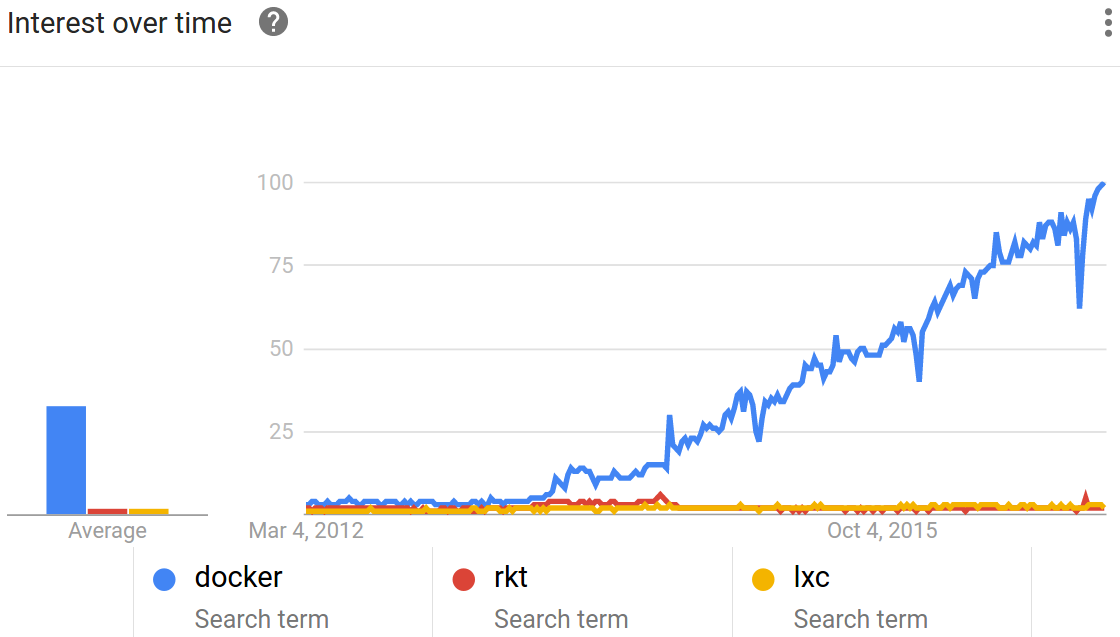
\includegraphics[width=0.9\linewidth]{img/google_trends_docker_rkt_lxc}
\caption[Google Trends for docker, rkt, lxc]{Google Trends for docker, rkt, lxc - wordwide, past 5 years, retrieved on 2017-02-27}
\label{fig:google_trends_docker_rkt_lxc}
\end{figure}

When containers are used to deploy applications, there is a requirement of certain orchestration tools which takes care of scheduling, resource allocation and availability. Popular container orchestration tools include Kubernetes, Docker Swarm, Mesosphere Marathon, Cloud Foundry Diego etc. Since all of them are open source projects, if we look at the number of stars on their GitHub repositories, Kubernetes turns out to be the most popular with 20964 stars at the time of writing \citep{github_stars_comparison}. Also, \cite{google_trends_kubernetes_docker_swarm} indicate the same.

For simplicity in implementation, it was decided to build a proof of concept with support for JavaScript applications and test the feasibility. 
\chapter{RESULTS}
%(i) progress made, (ii) results, (iii) sample code, (iv) refinement of the problem statement, and (v) potential work outline for the next 2-3 months. This will count for 25% of the final grade.                

%Upgrade the report of Stage 1, and add another chapter say called Results, which includes progress made, and the potential work outline for the next 2-3 months

After considering all the options, it was decided to build the platform using following technologies. Everything except GitHub are open source softwares. But, all the major open source activities in the world is carried out on GitHub.
\begin{itemize}
	\item \textbf{React}\footnote{\url{https://facebook.github.io/react/}} for user facing code console on browser
	\item \textbf{GitHub}\footnote{\label{github_website}\url{https://github.com/}} for storing all template environments as well as user code
	\item \textbf{Docker}\footnote{\url{https://www.docker.com/}} containers for deployment
	\item \textbf{Kubernetes}\footnote{\url{https://kubernetes.io/}} for container management and orchestration
	\item \textbf{Nginx}\footnote{\url{http://nginx.org/}} for reverse proxying urls to containers
\end{itemize}

\begin{figure}
	\centering
	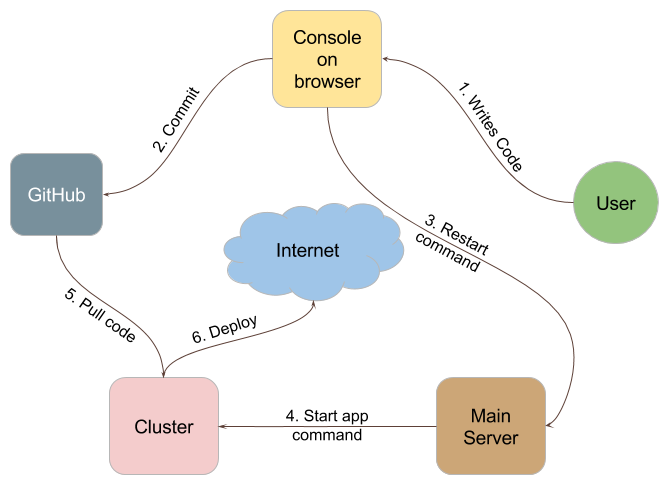
\includegraphics[width=0.9\linewidth]{img/user_flow}
	\caption[Overall flow diagram for the system]{Overall flow diagram for the system from user perspective}
	\label{fig:userflow}
\end{figure}

Fig.~\ref{fig:userflow} gives an overall view of the system. From a user perspective, the flow is as follows:
\begin{enumerate}
	\item User opens the console by going to the link created by administrators (say \textit{console.domain.com})
	\item User logs on to the console using GitHub credentials. This will link the user's GitHub account to the console
	\item All editable files are shown to the user on a side panel. In order to add more files, user goes to GitHub website and carry out necessary action
	\item User selects the file that has to be edited
	\item File is shown inside a code editor window where user can make any changes required
	\item Once the file is edited, user clicks on Commit \& Restart button
	\item User is shown a web link where the code's output (a webpage in this case) is displayed. This link is available on the internet (say \textit{user.app.domain.com})
	\item User can view logs for the code by clicking on the logs button
	
\end{enumerate}

\section{System Architecture}
The console and user applications are deployed to a cloud platform, Google Cloud\footnote{\url{https://cloud.google.com/}} in this case, as docker containers managed by Kubernetes (K8S) on a cluster of Virtual Machines (VM) running Container Linux OS\footnote{\url{https://coreos.com/}}. While the console is exposed as a web server where user logs in at \textit{console.domain.com}, all user application are exposed as \textit{user.app.domain.com}. Whenever a user issues command to run the code, the API server picks up corresponding code from GitHub and creates K8S objects, a service and deployment, on the cluster. K8S will put the code inside the pre-defined environment and starts a container. When a user visits \textit{user.app.domain.com}, the Nginx gateway, programmed using Lua, running on the cluster infers \textit{user} from the hostname and directs the connection to the right container. Inside the cluster, the containers are identified by internal, DNS lookups. Each container is assigned a hostname matching the user's name. A DNS server keeps track of these hostnames and resolves them to container IP addresses when necessary. 

The cluster where user appications are run comprises of many virtual machines. There is one master machine and many worker machines. They are all linked together using a private network and external access is through a loadbalancer which is guarded by a firewall. Only port 80 is exposed on the public IP address of the loadbalancer. On recieving a request, the loadbalancer delegates it to one of the worker machines using a round-robin algorithm. On each worker, a copy of Nginx gateway is running. This architecture is illustrated in Fig.~\ref{fig:systemarch}. 

\begin{figure}
\centering
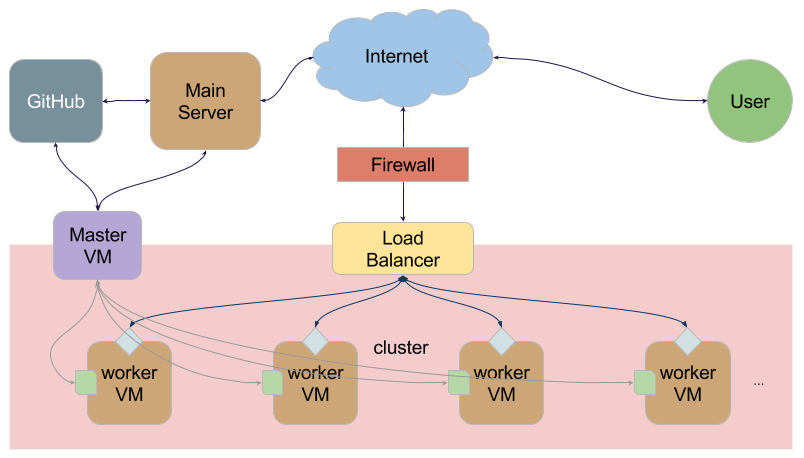
\includegraphics[width=0.9\linewidth]{img/system_arch}
\caption[Platform architecture]{Platform architecture indicating how a user interacts with main server, github and the application cluster}
\label{fig:systemarch}
\end{figure}

\section{Components}
Micoservices architecture \citep{dragoni_microservices:_2016} is adopted for the design and enigineering of components in the platform. This is in contrast to the typical monolithic software engineering practices that has been followed by the communinty and industy for a long time. Advantages fo a microservices architecture includes the ability to use multiple programming languages together and scale them individually without affecting other parts. Each microservice is deployed as a docker container, managed by K8S. Even the core K8S components are microservices which again run inside containers.

\subsection{Kubernetes}
Kubernetes is an open source cluster container management tool originally developed by Google \citep{burns_borg_2016} and later moved to Cloud Native Computing Foundation\footnote{\url{https://www.cncf.io/}}. It defines a set of primitives that collectively provide mechanisms for deploying maintaining and scaling applications through the use of containers. Docker conatiners are natively supported by K8S and support for rkt and lxc is under development.

The architecture of Kubernetes follows a master-slave layout. The key components can be divided to those manage each node and those reside in the master controller space. Fig.~\ref{fig:systeminternalarch} shows a brief overview of K8S architecure exploited for the current application. The key feature used here are \textit{\cite{deployments}} and \textit{\cite{services}} objects. Whenever a \textit{Deployment} object is created with required configuration, K8S starts a docker container with the given image name. The \textit{Service} object gives HTTP access to the container over a specified port and registers itself with DNS server. Objects are created over REST calls to the K8S API.

\begin{figure}
	\centering
	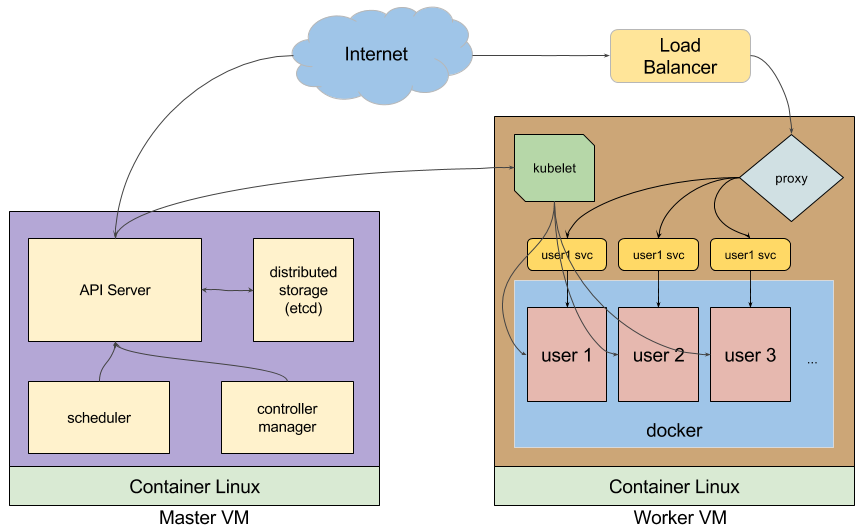
\includegraphics[width=0.9\linewidth]{img/system_internal_arch}
	\caption[Kubernetes architecture]{Kubernetes architecture indicting the controller components as well as user application running on a master-slave layout}
	\label{fig:systeminternalarch}
\end{figure}

Whenever an object is created or a change is made to an object, K8S logs it into its distributed storage system called \textit{etcd}\footnote{\url{https://coreos.com/etcd/}}. Another component called \textit{Controller Manager} is watching changes to \textit{etcd}. When a change is detected, it calculates the difference between the current state with desired state using a diff algorithm. Based on the output of these calculations, \textit{controller managers} executes actions through K8S API that will drive the system to desired state. This process is carried out in a loop such that $observe \rightarrow diff \rightarrow act$ cycles continue to happen forever and eventually drives the system to consistancy \citep{vogels_eventually_2009}.

\subsection{User Interface}
The React/Redux based user interface which runs on a web browser defines how a user interacts with the platform. The interface is designed to be simple and clutter free to direct focus on to the code only. A screenshot of the inteface is included in Fig.~\ref{fig:codeinterface} for clarity. Main components are a side bar where navigation and command controls are present and a main window where user and see and edit code. Links to view logs and lauch applicaitons are given on the top of sidebar. The main action button which says Commit \& Restart saves the changes to GitHub and refresh user application with new code. Below that, all editable files are shown, on which the user can click and it's content is shown available for editing on the right side. An open source code editor called ACE Editor\footnote{\url{https://ace.c9.io/}} is used for providing the coding interface. It supports syntax highlighting for a variety of languages as well as simple error highlighting.

\begin{figure}
	\centering
	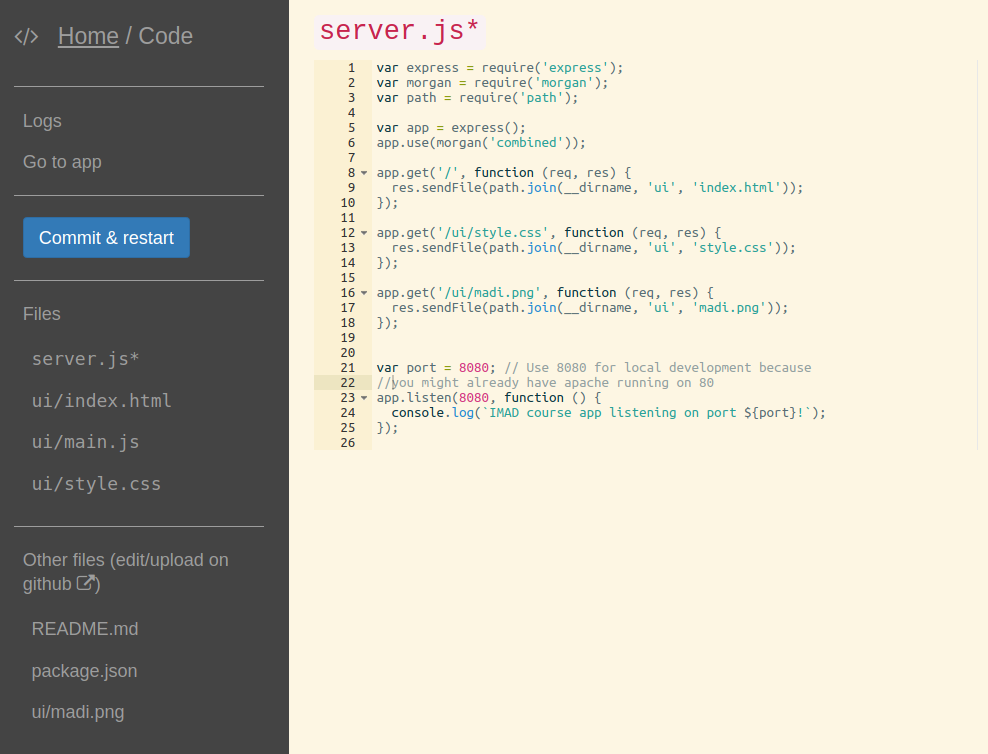
\includegraphics[width=0.9\linewidth]{img/code_interface}
	\caption[User interface]{The user interface of web app that is used to write and mange code}
	\label{fig:codeinterface}
\end{figure}

Non-editable or non-code files are shown as Other files. Updating them or adding new files can be done through GitHub website. This is deliberatly done so as to reduce complexity of the user interface. All edits to files are stored locally and saved directly to GitHub using GitHub API v3 \footnote{\url{https://developer.github.com/v3/}}.

\subsection{API Server}
The user interface communicates to an API server to carry out actions like starting or updating code of the user application, getting logs etc. API server is written using Node.js\footnote{\url{https://nodejs.org/en/}} and communicates with the K8S cluster via K8S API.
\subsection{Gateway and Reverse Proxy}
talk about gateway
\subsection{Programming Environment}
talk about env

\section{Issues and Solutions}

%%%%%%%%%%%%%%%%%%%%%%%%%%%%%%%%%%%%%%%%%%%%%%%%%%%%%%%%%%%%
% Appendices.

\appendix

\chapter{SOURCE CODE}

All source code is present in GitHub. Links are given here.
\begin{enumerate}
	\item User console\footnote{\url{https://github.com/hasura-imad/console}}
	\item API Server\footnote{\url{https://github.com/hasura-imad/api}}
	\item Nginx reverse proxy and gateway\footnote{\url{https://github.com/hasura-imad/gateway}}
	\item Base template for JavaScript environment\footnote{\url{https://github.com/hasura-imad/imad-app-v2}}
\end{enumerate}

%%%%%%%%%%%%%%%%%%%%%%%%%%%%%%%%%%%%%%%%%%%%%%%%%%%%%%%%%%%%
% Bibliography.

\begin{singlespace}
	\bibliography{refs}
\end{singlespace}


%%%%%%%%%%%%%%%%%%%%%%%%%%%%%%%%%%%%%%%%%%%%%%%%%%%%%%%%%%%%
% List of papers

\listofpapers

\begin{enumerate}  
\item Authors....  \newblock
 Title...
  \newblock {\em Journal}, Volume,
  Page, (year).
\end{enumerate}  

\end{document}
